% compile using the following sequence of commands:
% pdflatex writeup
% bibtex writeup
% pdflatex writeup
% pdflatex writeup

% basic setup:
\documentclass[12pt, titlepage]{article}
\usepackage[utf8]{inputenc}
\usepackage[letterpaper, margin=1in]{geometry}
\usepackage{setspace}
\usepackage{amsmath}
\usepackage{siunitx}
\usepackage[]{graphicx}
\graphicspath{{./resources/}}
\usepackage{booktabs}
\usepackage{longtable}
%\usepackage{hyperref}

% fix tilde:
\newcommand{\textapprox}{\raisebox{0.5ex}{\texttildelow}}

% set up bibliography:
\usepackage[backend=bibtex, style=phys]{biblatex}
\addbibresource{citations.bib}

% change title sizes:
\usepackage{titlesec}
\titleformat*{\section}{\large\bfseries}
\titleformat*{\subsection}{\bfseries}

% change table of contents formatting:
\usepackage{tocloft}
\renewcommand{\cfttoctitlefont}{\large\bfseries}
\renewcommand{\cftsecfont}{\normalsize}
\renewcommand{\cftsubsecfont}{\normalsize}

% title page information:
\title{\Large Anodic and Cathodic Polarization of 1018 Mild Steel \\
		and 304 Stainless Steel \\
		\bigskip
	\normalsize MSE 130: Experimental Materials Science and Design}
\author{\normalsize Jonathan Lee \\
	\normalsize Department of Materials Science and Engineering \\
	\normalsize University of California, Berkeley}
\date{\normalsize 18 October 2020}

\begin{document}

\maketitle

\setcounter{page}{2}

\tableofcontents

\doublespacing

\newpage

\section{Abstract}

A series of polarization cell experiments were conducted so as to characterize the corrosion behavior of 1018 mild steel and 304 stainless steel samples when polarized in strongly-acidic solutions, on behalf of an anonymous manufacturer.  Three models of varying complexity were employed to fit the data, including a nontraditional modification of the Butler-Volmer equation that incorporated diffusion limitations and the synthesis of passivation barriers.  It was found that for the H/Fe redox couple on 1018MS, $j_{\text{corr}} = 1.49$e-6 A/mm$^2$ and $\Delta \phi_{\text{corr}} = -0.491$ V vs. SCE.  For 304SS in 1M H$_2$SO$_4$ solution, the passivation barrier was found to form at -0.277 V and break down at 0.892 V, while in 1M HCl solution, the barrier formed at -0.157 V and broke down at 0.402 V due to chloride pitting.

\section{Introduction}

- the purpose of this report is to quantify the corrosion behavior of rod samples of 1018 mild carbon steel (1018MS +composition) and 304 stainless steel (304SS + composition) in strongly acidic solutions (1M HCl and 1M H2SO4), as submitted by an anonymous manufacturer for quality-control purposes.

- discussion of what happens when a metal is placed in solution with a counter-electrode to maintain neutrality - dissolution equilbrium potential (equal currents) difference with solution wrt the solution potential (encoded as voltage wrt the reference electrode) as given by the butler-volmer equation, with the cofactor given by <eqn> representing the oft-cited metric of the Tafel Slope, which may be understood as the relationship between overpotential (eta) and the resulting ln(i); and the intersection (zero current) representing the equilibrium potential that develops

- this behavior is modified by additional redox half-reactions that may now take place involving species in solution, which makes possible coupling between redox half-reactions involving different species

- in the case of mild steels in acidic solution, we are particularly interested in the coupling between the H+ reduction reaction and the Fe oxidation reaction (C in alpha-phase is negligible); in this case and in others when a metal dissolves into solution by coupling with a solution species, the resulting equilibrium potential is often referred to as the corrosion potential (m del s phi); potentials lower than the corrosion potential are called the "cathodic" regime because current must be supplied to the reaction, while potentials higher than the corrsion potential are the "anodic" regime, and the whole sweep is called the polarization curve of the material

- in the local vicinity (colloqually considered as +- 100 mV) of the corrosion potential, behavior is expected to closely match that predicted by the bulter-volmer equation, but at larger potentials, the half-reaction may become diffusion limited (for example, by the formation of a polarized double-layer on the electrode surface); in these cases, the manifested current is depressed relative to the butler-volmer prediction; we may rudimentarily model this scenario by modifying the relevant butler-volmer term with a resistive component, producing (modified eqn)

- 1018MS is expected to further deviate from the behavior predicted by (bv and mod-bv) by virtue of its microstructure; 0.18 wt% C means X wt% Fe3C and (1-X) wt% alpha, which by virtue of cooling through the alpha+gamma sub-eutectoid region will manifest as Y wt% ferritic alpha-phase and (1-Y) wt% pearlite of composition #### -- Fe3C does not dissolve as the alpha-phase does, yet conducts metallically and catalyzes the reactions of the H/H+ redox couple by means of offering a much higher exchange current density (i0 in the bulter-volmer eqn) than on ferrite; this means that as the corrosion progresses and the Fe3C cementite lamellae are "excavated," we might expect the H+ reduction reaction to increase in rate

- 304 SS is expected to further deviate from the behavior predicted by (bv and mod-bv) by virtue of its engineered passivation behavior; namely, at a second threshold potential above the H/Fe corrosion potential, the Cr content oxidizes to form a "passivation layer" consisting largely of Cr2O3 (but other compounds too); this passivation layer may be considered as an extremely effective diffusion barrier, i.e. one in which the resistive terms of eqn (mod-bv) is enormous, producing an ohmic I/V response that is nearly flat

- at the even-higher "breakdown potential," the passivation layer may oxidize (eqn given in text), restoring the diffusion-limited Fe oxidation behavior after fully ablating; the breakdown potential may be slightly differentiated from the equilbrium potential of the Cr III/Cr VI redox couple

- at the even-even-higher water breakdown potential, most of the current response comes from the decomposition of H2O into oxygen gas (which is relatively insoluble in these acidic solutions), hydrogen ions, and electrons

- 304SS also manifests a particular behavior in HCl: chrloride ions attack the passivation later in a self-catalyzed reaction, eating through the layer in local regions; this occurs at a lower potential than the breakdown potential and is called the "pitting potential"

- therefore in order to characterize the manufacturer's submitted samples, the goal is to quantify the following:
	1. 304SS: corrosion poten, local H/Fe tafel slopes, passivation poten, pitting poten in HCl, breakdown poten, Cr equilibrium poten, water breakdown poten
	2. 1018MS: corrosion poten, local H/Fe tafel slopes, effect of cementite microstructure evolution


\section{Experimental Procedure}

1/8" diameter rods of 304SS and 1018MS were cut into cylindrical samples, then sanded with 600-grit paper and rinsed with deionized water so as to clean their surfaces.\cite{labguide}  In total, four samples were produced (2x 304SS and 2x 1018MS).  The samples were imaged under an optical microscope so as to provide a reference against which to compare their corroded surfaces.

Each sample was installed as the working electrode within a polarization cell, alongside a platinum counter-electrode and a saturated calomel reference electrode (SCE).  So as to minimize the effects of solution resistivity on the measured voltage, the reference electrode was contained within a Lugger-Habin probe, of which the capillary tip was placed at the midpoint of the sample.  The polarization cell was filled with either 250 mL of 1M HCl solution or 250 mL of 1M H2SO4 solution.  The Luggin-Haber probe was filled with the same chosen solution to a surface level 1/4" below that of the polarization cell; this precluded the contamination of the polarization cell with 4M Cl- solution from the SCE reference.  Care was taken during filling to avoid bubbles, as well as to position the Luggin-Haber probe in a way that would not allow bubbles to enter its capillary during the course of the experiment.\cite{labguide}  Sample dimensions, solutions, and immersion lengths are recorded in Table \ref{table:samples}.

\begin{table}[h!]
	\centering
	\begin{tabular}{lcccc}
	\toprule
	Sample & Materials & Soln & Diameter & Immersed Length \\
	\midrule
	1 & 1018MS & H$_2$SO$_4$ & 3.12 mm & 14.8 mm \\
	2 & 1018MS & HCl	 & 3.12 mm & 15.6 mm \\
	3 & 304SS  & H$_2$SO$_4$ & 3.12 mm & 16.1 mm \\
	4 & 304SS  & HCl	 & 3.12 mm & 13.6 mm \\
	\bottomrule
	\end{tabular}
	\caption{Sample dimensions used to calculate critical current densities from the collected current data.}
	\label{table:samples}
\end{table}

\begin{table}[h!]
	\centering
	\begin{tabular}{lccp{2.5cm}p{2.5cm}p{6cm}}
	\toprule
	Scan & Sample & Solution & Classification & Sweep Rate (mV/sec) \\
	\midrule
	0 & 1018MS & H2SO4 & Ano/Cat & 10 mV/sec \\
	1 & 1018MS & H2SO4 & LPR & 1 mV/sec \\
	2 & 1018MS & H2SO4 & Ano/Cat & 10 mV/sec  \\
	3 & 1018MS & H2SO4 & LPR & 1 mV/sec  \\
	4 & 1018MS & HCl & Ano/Cat & 10 mV/sec  \\
	5 & 1018MS & HCl & LPR & 1 mV/sec  \\
	6 & 1018MS & HCl & Ano/Cat & 10 mV/sec  \\
	7 & 1018MS & HCl & LPR & 1 mV/sec \\
	8 & 304SS & H2SO4 & Cathodic & 10 mV/sec \\
	9 & 304SS & H2SO4 & Anodic & 10 mV/sec  \\
	10 & 304SS & HCl & Cathodic & 10 mV/sec  \\
	11 & 304SS & HCl & Anodic & 10 mV/sec  \\
	\bottomrule
	\end{tabular}
	\caption{General description of the 12 collected polarization curves.}
	\label{table:sweeps}
\end{table}

The three electrodes were connected to a potentiostat constructed by previous laboratory personnel (10V compliance voltage, 190 mA maximum current, 200 mA thermal fuse cutoff, 15pA reference input current, 1e-6 mA current sensitivity, 2\% current accuracy).\cite{labguide, gsi}  The approximate location of the H/Fe corrosion potential was identified, after which various polarization sweeps were conducted for each sample.  Twelve polarization sweeps were collected in total; the overall classification of each sweep are enumerated in Table \ref{table:sweeps}.  The parameters of each type of sweep were:

\begin{itemize}

	\item 1018MS Anodic/Cathodic Sweep (``AnoCat''): upward scan from 200 mV below $\Delta \phi_{\text{corr}}$ to the potential above $\Delta \phi_{\text{corr}}$ that produced 1 mA anodic current, followed by a reverse scan to return to the starting potential.
	\item 1018MS Linear Polarization Resistance Sweep (``LPR''): immediately after an Ano/Cat sweep, potential help had 200 mV below $\Delta \phi_{\text{corr}}$ until the current stabilized; after which an upward scan from 20 mv below $\delta \phi_{\text{corr}}$ to 20 mv above $\delta \phi_{\text{corr}}$ and back was performed.
	\item 304SS Cathodic Sweep: downward scan from 20 mV above $\Delta \phi_{\text{corr}}$ to 700 mV below $\Delta \phi_{\text{corr}}$.
	\item 304SS Anodic Sweep: upward scan from 20 mV below $\Delta \phi_{\text{corr}}$ to the potential that achieved the maximum potentiostat current of 190 mA, followed by a downward scan until a transition to cathodic behavior was observed.\cite{labguide}

\end{itemize}

It should be noted that the 304SS Anodic sweep in HCl required reversing the scan direction in the vicinity of 100 mA instead of near the maximum potentiostat current, since Cl$^-$ pitting was predicted to produce a rise in current even after the potential was decreased.\cite{labguide}

After the sweeps were concluded, the samples were dried and imaged once more under an optical microscope at magnifications of 5x, 10x, and 20x.  Microscopy images are contained within Appendix 2.



\section{Results}

\subsection{1018MS Corrosion Parameters from Anodic/Cathodic Sweeps}

	\begin{figure}[h!]
		\centering
		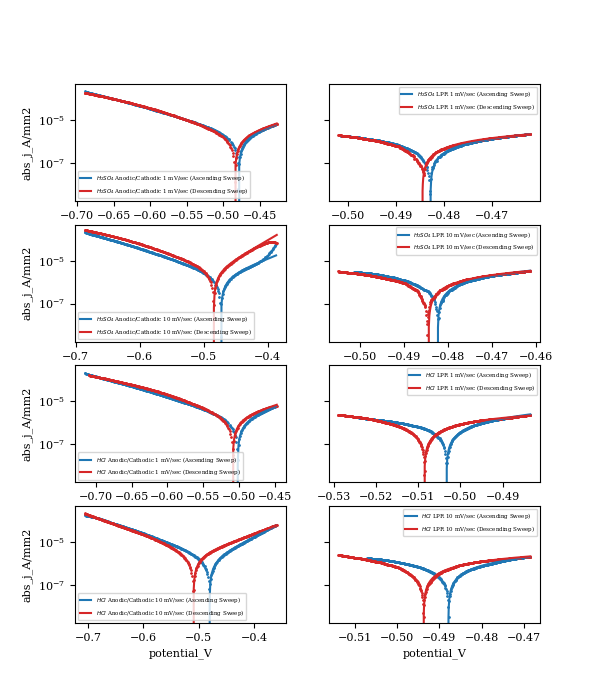
\includegraphics[width=5.0in]{resources/fig_2b.png}
		\caption{Results of fitting Equation \ref{eqn:bv_tafel} to the eight 1018MS polarization sweeps.  The scales of the axes indicate little variation in the current densities and potentials relative to SCE among the sweeps, though the limited scope of the LPR sweeps produced a large variance in their calculated parameters.}
		\label{fig:anocat}
	\end{figure}

	\begin{table}[h!]
		\centering
		\begin{tabular}{lllrrrr}
\toprule
  &     &     &  $A_{\text{H}}$ (V) &  $A_{\text{Fe}}$ (V) &  $j_{\text{corr}}$ (A/mm$^2$) &  $\Delta \phi_{\text{corr}}$ (V) \\
Scan & Soln & Dir &                     &                      &                               &                                  \\
\midrule
0 & H$_2$SO$_4$ & Asc &          -8.778e-02 &            8.903e-02 &                     1.784e-06 &                       -4.794e-01 \\
  &     & Des &          -9.588e-02 &            8.833e-02 &                     1.888e-06 &                       -4.843e-01 \\
2 & H$_2$SO$_4$ & Asc &          -8.341e-02 &            8.519e-02 &                     1.663e-06 &                       -4.730e-01 \\
  &     & Des &          -5.730e-02 &            8.076e-02 &                     3.096e-06 &                       -4.842e-01 \\
4 & HCl & Asc &          -7.706e-02 &            8.553e-02 &                     1.277e-06 &                       -5.022e-01 \\
  &     & Des &          -9.978e-02 &            8.326e-02 &                     1.765e-06 &                       -5.090e-01 \\
6 & HCl & Asc &          -7.490e-02 &            9.225e-02 &                     1.469e-06 &                       -4.806e-01 \\
  &     & Des &          -1.035e-01 &            8.415e-02 &                     2.140e-06 &                       -5.097e-01 \\
\bottomrule
\end{tabular}

		\caption{Derived parameters for Equation \ref{eqn:bv_tafel} (Tafel slopes, corrosion currents, and corrosion potentials relative to SCE) for 1018MS anodic/cathodic sweeps.  See Appendix 2 for associated variances.}
		\label{table:anocat}
	\end{table}

All collected 1018MS polarization sweeps were fit to the form of Equation \ref{eqn:bv_tafel} using the Python package \textit{lmfit}.\cite{lmfit}  Since Equation 1 does not account for diffusion-limited behavior, each fitting was performed within a narrow data window of width 100 mV centered on the corrosion potential.  The quality of fits varied: while the parameters derived from the LPR scans possessed much smaller variances due to their greater data densities, the parameters derived from the Ano/Cat scans were far more consistent in terms of value.  The fitted parameters and variances from the designated Ano/Cat scans are presented in Table \ref{table:anocat}, while the according fits are plotted against the data in Figure \ref{fig:anocat}.  All fitted parameters for the eight 1018MS scans, as well as their variances, may be found in Appendix 2.

Using solely the data from the Ano/Cat scans (Scans 0, 2, 4, and 6), the average values of the Tafel slopes were found to be $A_{\text{H}} = -8.620$e-02 V and $A_{\text{Fe}} = 8.606$e-02 V; the similarity in the magnitude of these values supports the assumption that $\beta \approx 0.5$ in Equation \ref{eqn:bv_raw}.  The average corrosion potential was found to be $\Delta \phi_{\text{corr}} = -0.4903$ V vs. SCE, with the associated average corrosion rate being $j_{\text{corr}} = 1.88$e-6 A/mm$_2$.  The variances in the equilibrium parameters were much smaller than their respective values ($\sigma^2(j_{\text{corr}}) = 2.14$e-15 A/mm$^2$, $\sigma^2(\Delta \phi_{\text{corr}}) = 5.41$e-8 V), but the variances of the Tafel slopes were found to be uncharacteristically large ($\sigma^2(A_{\text{H}}) = 99.5$ V, $\sigma^2(A_{\text{Fe}}) = 159$ V).  Given the similarities of the actual fitted parameters, however, this was though to be an error in statistical estimation rather than an indicator of actual variance in the Tafel slopes.

It should be noted that, in this analysis, variances were propagated using:

	\begin{equation}
		f(a_1, a_2, ...) \rightarrow \sigma^2_f = \sum_i \left( \frac{\partial f}{\partial a_i} \right)^2 \sigma^2_{a_i}
		\label{eqn:se}
	\end{equation}

It should also be noted that hystersis was observed within these scans; the observed corrosion potentials on the downward half of the sweeps were consistently lower than those of the upward halves.  A discussion of this hystersis is reserved for the Discussion.

\subsection{1018MS Corrosion Parameters from LPR Sweeps}

	\begin{table}[h!]
		\centering
		\begin{tabular}{llllrrrr}
\toprule
  &     &           &     &  $j_{corr}$ (A/mm$^2$) &  $\Delta \phi_{corr}$ (V) &  $\sigma^2(j_{corr})$ &    n \\
Scan & Soln & Rate & Dir &                        &                           &                       &      \\
\midrule
1 & H$_2$SO$_4$ & 1 mV/sec & Asc &              1.342e-06 &                -4.830e-01 &             6.559e-16 &  338 \\
  &     &           & Des &              1.354e-06 &                -4.841e-01 &             3.434e-15 &  421 \\
3 & H$_2$SO$_4$ & 10 mV/sec & Asc &              2.058e-06 &                -4.822e-01 &             2.552e-15 &  342 \\
  &     &           & Des &              1.941e-06 &                -4.849e-01 &             1.070e-14 &  444 \\
5 & HCl & 1 mV/sec & Asc &              1.302e-06 &                -5.032e-01 &             4.275e-14 &  353 \\
  &     &           & Des &              1.335e-06 &                -5.085e-01 &             2.300e-14 &  442 \\
7 & HCl & 10 mV/sec & Asc &              1.265e-06 &                -4.879e-01 &             4.494e-15 &  342 \\
  &     &           & Des &              1.297e-06 &                -4.937e-01 &             2.720e-14 &  443 \\
\bottomrule
\end{tabular}

		\caption{Fitting parameters for Equation \ref{eqn:bv_lpr}, as calculated from the LPR scans for 1018MS.  The fitting package \textit{lmfit} was unable to estimate the variance for $\Delta \phi_{\text{corr}}$.}
		\label{table:lpr}
	\end{table}

	\begin{figure}[h!]
		\centering
		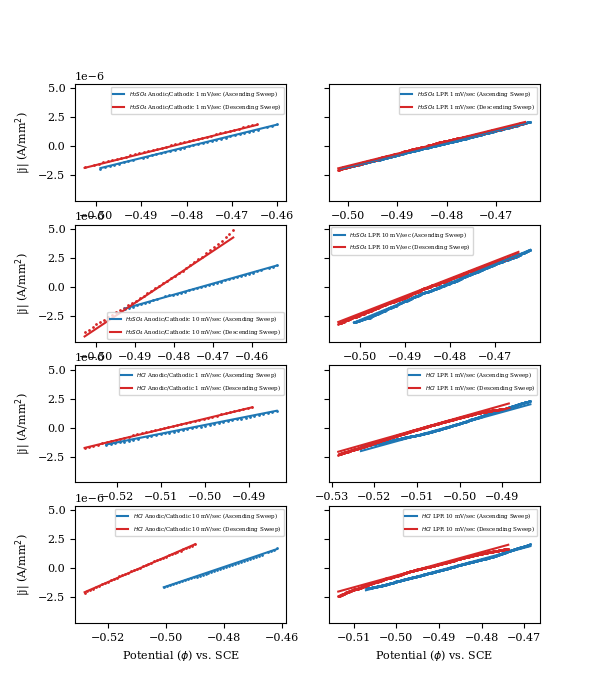
\includegraphics[width=5.0in]{resources/fig_2c.png}
		\caption{Linear fits in the low-overpotential regime for all eight 1018MS scans.}
		\label{fig:lpr}
	\end{figure}

Figure \ref{fig:lpr} shows the results of fitting Equation \ref{eqn:bv_lpr} to local linear regions of each of the 1018MS scans.  In the case of the dedicated LPR scans, this region comprised the entirity of the scans, while the Ano/Cat scans were trimmed to a window of $\Delta \phi_{\text{corr}} \pm 20$ mV in order to isolate a comparable region.  All 1018MS scans were found to possess linear behavior in the vicinity of $\Delta \phi_{\text{corr}}$, validating the LPR measurement approach.  The resulting parameters from the pre-designated LPR scans (Scans 1, 3, 5, and 7) are shown in Table \ref{table:lpr}, while the fitted parameters for all eight 1018MS scans are presented in Appendix 3.

Using these data, the average value for the corrosion current was found to be 1.49e-6 A/mm$^2$, with an associated variance of $\sigma^2(j_{\text{corr}}) = 1.79$e-15 A/mm$^2$.  The average value of the corrosion potential was found to be -4.910 V, though \textit{lmfit} estimated the variances of this parameter to be 0.

\subsection{Deconvolution of 304SS H$_2$SO$_4$ Polarization Sweep}

In order to analyze the 304SS polarization curves, the anodic and cathodic sweeps were concatenated.  In the case of the HCl curves, this did not require any modification; however, the cathodic H$_2$SO$_4$ curve exhibited a corrosion potential \textapprox 0.25 V higher than any other corrosion potential measured in this experiment.  This was assumed to be an experimental error; sa such, the data were shifted so that their corrosion potential aligned with that of the anodic curve.

For both the H$_2$SO$_4$ and HCl curves, the hydrogen reduction reaction was fit to the diffusion-limited model (Equation \ref{eqn:bv_w}) and subtracted out of the remaining data.  This was observed, however, to have little effect.  In particular, this deconvolution did not remove any other singularities or depressions in the curves, indicating that other reduction reactions were active within certain $\phi$-regimes.  The dominant reactions in portions of the H$_2$SO$_4$ curve were thus explained as follows:

\singlespacing
\begin{itemize}
	\item \textbf{$<$ \textapprox -0.4 V:} $2 \text{H}^+ + 2 e^- \rightarrow \text{H}_2$ (reduction of hydrogen ions to produce hydrogen gas, as evidenced by bubbling on the electrode surface)
	\item \textbf{\textapprox -0.4 V to \textapprox -0.3 V:} $\text{Fe} \rightarrow \text{Fe}^{2+} + 2 e^-$ (oxidation and dissolution of iron)
	\item\textbf{\textapprox -0.3 V to \textapprox 0 V:} $\text{Cr} \rightarrow \text{Cr}^{3+} + 3 e^-$ (passivation of electrode surface due to formation of Cr$_2$O$_3$, and intersection with an unknown reduction reaction, such as the reduction of acqueous Fe, Ni, or Cr)
	\item\textbf{\textapprox 0 V to \textapprox 0.9 V:} $\text{Cr} \rightarrow \text{Cr}^{3+} + 3 e^-$ (passivation of electrode surface due to formation of Cr$_2$O$_3$)
	\item\textbf{\textapprox 0.9 V to \textapprox 1.5 V:} $\text{Cr}^{3+} \rightarrow \text{Cr}^{6+} + 3 e^-$ (destruction of passivation layer to formation of aqueous HCrO$_4^-$, as evidenced by reddish-orange ion trails surrounding the electrode)
	\item \textbf{$>$ \textapprox 1.5 V:} $\text{H}_2\text{O} \rightarrow 2 \text{H}^+ + \frac{1}{2} \text{O}_2 + 2 e^-$ (breakdown of water, as evidenced by renewed bubbling on the electrode surface)
	\item \textbf{$<$ \textapprox 0.8 V on descending sweep:} $\text{Cr}^{6+} + 3 e^- \rightarrow \text{Cr}^{3+}$ (reduction of aqueous Cr to reconstruct the passivation layer)

\end{itemize}
\doublespacing

An attempt was then made to deconvolute the H$_2$SO$_4$ curve into contributions from its component reactions, as modelled using Equation \ref{eqn:bv_w}.  It was found, however, that Equation \ref{eqn:bv_w} could not fit the passivation region; furthermore, the presence of multiple singularities precluded a traditional stepwise model of the passivation potential, which would not be able to manifest the changes in concavity required to replicate these singularities.  Equation \ref{eqn:bv_w} was therefore modified by means of a changing resistivity:

	
	\begin{equation}
		\rho = \rho_{\text{lim}} + 
		\rho_{\text{pass}} \left[
			1 - \exp (- \alpha_{\text{pass}} \eta_{\text{pass}}^3) \right]
		\label{eqn:rho_jmak}
	\end{equation}

	\begin{table}[h!]
		\centering
		\begin{tabular}{lrrrr}
\toprule
{} &  $\phi_0$ (V) &  $j_0$ (A/mm$^2$) &    $A$ (V) &  $\rho_{\text{lim}}$ ($\Omega \cdot$mm) \\
Reaction                             &               &                   &            &                                         \\
\midrule
H$^+$ reduction                      &    -3.728e-01 &        -9.612e-08 & -1.138e-01 &                               1.587e+02 \\
Fe oxidation (passivation-limited)   &    -3.927e-01 &         7.891e-07 &  3.505e-03 &                               3.905e+04 \\
Cr$_2$O$_3$ barrier breakdown (asc)  &     9.688e-01 &         9.902e-07 &  3.701e-02 &                               1.968e+03 \\
H$_2$O breakdown (asc)               &     1.596e+00 &         1.065e-04 &  2.025e-01 &                              3.230e-312 \\
unknown reduction reaction           &     1.500e-01 &        -5.000e-11 & -3.289e-02 &                               2.000e+05 \\
Cr$_2$O$_3$ solution deposition      &     1.070e+00 &       -1.812e+169 & -9.784e-06 &                               4.502e+06 \\
Cr$_2$O$_3$ barrier breakdown (desc) &     9.814e-01 &         4.565e-07 &  5.713e-02 &                               1.324e+03 \\
H$_2$O breakdown (desc)              &     1.599e+00 &         1.016e-04 &  1.971e-01 &                               3.765e-06 \\
\bottomrule
\end{tabular}

		\begin{tabular}{lrrr}
\toprule
{} &  $\phi_{pass}$ (V) &  $\alpha_{pass}$ (V$^{-3}$) &  $\rho_{pass}$ ($\Omega \cdot$mm) \\
Reaction                             &                    &                             &                                   \\
\midrule
Fe oxidation (passivation-limited)   &         -3.530e-01 &                   4.814e+00 &                         6.966e+06 \\
Cr$_2$O$_3$ barrier breakdown (asc)  &          1.300e+00 &                   8.971e-03 &                         5.670e+07 \\
unknown reduction reaction           &         -3.000e-02 &                   1.000e+01 &                         1.000e+07 \\
Cr$_2$O$_3$ barrier breakdown (desc) &          1.239e+00 &                   7.470e-03 &                         2.868e+07 \\
\bottomrule
\end{tabular}

		\caption{Deconvolution parameters for Equation \ref{eqn:bv_w} from the combined anodic/cathodic H$_2$SO$_4$ polarization sweep.  Four fitting regions required the JMAK resisitity modification outlined in Equation \ref{eqn:rho_jmak}.}
		\label{table:h2so4_deconv}
	\end{table}

	\begin{figure}[h!]
		\centering
		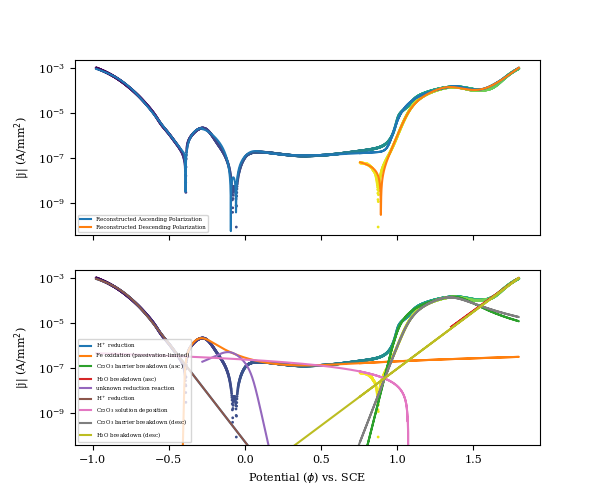
\includegraphics[width=5.0in]{resources/fig_2a1.png}
		\caption{Top: Fitted H$_2$SO$_4$ curves generated by deconvolution procedure.  Bottom: Individual reaction components fitted using Equations \ref{eqn:bv_w} and \ref{eqn:rho_jmak}.}
		\label{fig:h2so4_deconv}
	\end{figure}
This ``ansatz'' treats the passivation layer as an additional resistivity in series with that of the diffusion layer.  Its two-dimensional formation is modeled using Johnson-Mehl-Avrami-Kolmogorov kinetics.\cite{labguide_1}  Since the potential ramp rate is constant throughout the curve, time in the JMAK equation was replaced with the overpotential relative to the passivation potential ($\eta_{\text{pass}}$).  Such a form produces an s-curve that, while having no rigorous theoretical basis, nevertheless provides an improved fitting approximation of regions of the polarization curve.  The results of the deconvolution of the H$_2$SO$_4$ into individual reaction components are presented in Table \ref{table:h2so4_deconv}, while the resulting curves are presented in Figure \ref{fig:h2so4_deconv}.

From this analysis, the passivation potential $\Delta \phi_{\text{pass}}$ might be defined as the ``nucleation'' potential for the passivation barrier described in Equation \ref{eqn:rho_jmak}.  For the case of H$_2$SO$_4$, this was fitted as -0.353 V.  Meanwhile, a more conventional approach might be to consider the passivation potential as the potential corresponding to the maximum observed dissolution rate; in this case, this is -0.277 V, corresponding to a dissolution rate of 2.15e-6 A/mm$^2$.  It should further be noted that the end of the passivation regime may be quantified by the crossover corresponding to the Cr III/Cr VI redox couple on the reverse-sweep, fitted to be 0.892 V vs. SCE.  This value is 9.99\% below the the literature value (0.991 V vs. SCE).

\subsection{Deconvolution of 304SS HCl Polarization Sweep}

Following the same procedure as with the H$_2$SO$_4$ sweep, the dominant reactions over the course of the HCl curve were proposed to be:

\singlespacing
\begin{itemize}
	\item \textbf{$<$ \textapprox -0.4 V:} $2 \text{H}^+ + 2 e^- \rightarrow \text{H}_2$ (reduction of hydrogen ions to produce hydrogen gas, as evidenced by bubbling on the electrode surface)
	\item \textbf{\textapprox -0.4 V to \textapprox 0.2 V:} $\text{Fe} \rightarrow \text{Fe}^{2+} + 2 e^-$ (oxidation and dissolution of iron)
	\item\textbf{\textapprox 0.2 V to \textapprox 0.3 V:} $\text{Cr} \rightarrow \text{Cr}^{3+} + 3 e^-$ (passivation of electrode surface due to formation of Cr$_2$O$_3$)
	\item\textbf{$>$ \textapprox 0.3 V:} destruction of passivation layer though Cl$^-$ pitting
	\item\textbf{$<$ \textapprox 0.5 V on descending:} autocatalytic Cl$^-$ pitting (eventual restoration of passivation barrier)
\end{itemize}
\doublespacing

The resulting fitting parameters are summarized in Table \ref{table:hcl_deconv}, while the deconvolved curves are presented in Figure \ref{fig:hcl_deconv}.  The fitted corrosion potential was found to be -0.164 V, while the maximum Fe corrosion rate of 8.43e-4 A/mm$^2$ appeared at -0.157 V vs. SHE.  No post-passivation singularities were observed.

	\begin{table}[h!]
		\centering
		\begin{tabular}{lrrrr}
\toprule
{} &  $\phi_0$ (V) &  $j_0$ (A/mm$^2$) &    $A$ (V) &  $\rho_{lim}$ ($\Omega \cdot$mm) \\
Reaction                           &               &                   &            &                                  \\
\midrule
H$^+$ reduction                    &    -3.478e-01 &        -3.793e-07 & -1.145e-01 &                        3.210e+02 \\
Fe oxidation (diffusion-limited)   &    -4.695e-01 &         1.498e-08 &  3.570e-02 &                        2.157e+03 \\
Fe oxidation (passivation-limited) &    -4.695e-01 &         1.498e-08 &  3.570e-02 &                        2.157e+03 \\
Cl$^-$ ion pitting                 &     3.928e-01 &         8.802e-05 &  4.837e-02 &                        9.837e+01 \\
\bottomrule
\end{tabular}

		\begin{tabular}{lrrr}
\toprule
{} &  $\phi_{pass}$ (V) &  $\alpha_{pass}$ (V$^{-3}$) &  $\rho_{pass}$ ($\Omega \cdot$mm) \\
Reaction                           &                    &                             &                                   \\
\midrule
Fe oxidation (passivation-limited) &         -1.643e-01 &                   5.187e+03 &                         5.946e+03 \\
\bottomrule
\end{tabular}

		\caption{Deconvolution parameters for Equations \ref{eqn:bv_w} and \ref{eqn:rho_jmak} from the combined anodic/cathodic H$_2$SO$_4$ polarization sweep.}
		\label{table:hcl_deconv}
	\end{table}


	\begin{figure}[h!]
		\centering
		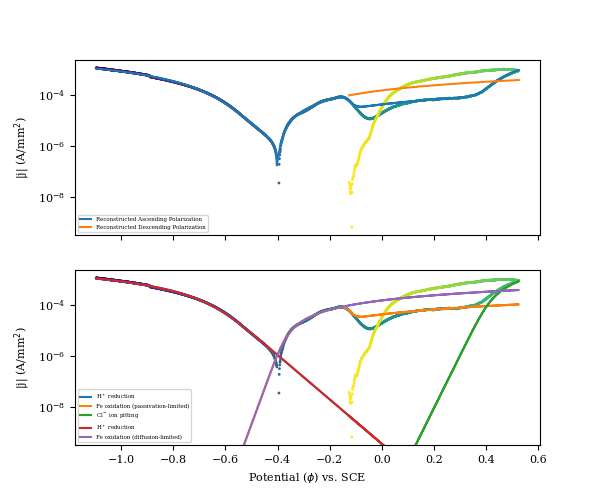
\includegraphics[width=5.0in]{resources/fig_2a2.png}
		\caption{Top: Fitted HCl curves generated by deconvolution procedure.  Bottom: Individual reaction components fitted using Equations \ref{eqn:bv_w} and \ref{eqn:rho_jmak}.}
		\label{fig:hcl_deconv}
	\end{figure}




\section{Discussion}

\subsection{Comments Upon Fitting Procedure Validity}

In the above analyses, three different fitting procedures were deployed: (1) a Butler-Volmer equation using Tafel slopes, as described by Equation \ref{eqn:bv_tafel}; (2) a linearized Butler-Volmer equation applied in the low-$\eta$ limit following Equation \ref{eqn:bv_lpr}; and (3) a generalized diffusion and passivation half-reaction model described by Equations \ref{eqn:bv_w} and \ref{eqn:rho_jmak}.  Of the three, only the linearized model appears to produce consistent and reliable results, as qualified by the low variances of its fitted parameters.

The Tafel-slope equation produced consistent results across multiple scans, but a possible fitting artifact produced variances that were several orders of magnitude larger than the parameters themselves.  This might be attributed to the fact that variances lose meaning when applied to non-linear and non-gaussian models; a better way of parameterizing uncertainty in such situations might be to introduce Monte Carlo noise into the dataset.\cite{montecarlo}

Meanwhile, the decision was made not to estimate variances for the 304SS deconvoluted curves.  The author wishes to emphasize that this procedure was highly subjective in nature; the results depended heavily on the initial seed parameters provided to \textit{lmfit}.  The deconvolution was nevertheless an instructive exercise; the model may have utility in the future design of a rigourous fitting algorithm.

\subsection{Discussion of Hysteresis in 1018MS Curves}

As seen in Figure \ref{fig:anocat}, the 1018MS Ano/Cat and LPR curves all exhibited hysteresis between the upward and downward portions of the sweep; the downward portion consistently manifested a more-negative corrosion potential.

Recalling the discussion in the Introduction regarding the microstructure of 1018MS, one might attempt to explain this hysteresis via hydrogen reduction catalysis by the exposed Fe$_3$C lamellar microstructure.  The hystersis, however, runs in direct contradiction to the predicted effects of such a catalysis, which would enhance the exchange current density of the reduction reaction and elevate the current at potentials more negative than $\Delta \phi_{\text{corr}}$.  As a result, $\Delta \phi_{\text{corr}}$ would shift to more positive values, since the catalyzed H$^+$ reduction reaction would be able to match the rate of Fe oxidation at a lower driving force.  Yet the hystersis manifests as a shift in the opposite direction, implying that it is the exchange current of Fe oxidation that has instead been elevated.

One possible mechanism to explain this behavior would be the formation of a passivating oxide on the sample surface in between polarization sweeps.  Such a layer would depress the exchange current density of the Fe reduction reaction on the upward sweep, but once it had been ablated by vigorous Fe corrosion at positive overpotentials, it would no longer effect the exchange current density.  As such, the exchange current density on the down-sweep would appear elevated.  It is also possible that the alloying Mn in the 1018MS plays a role, though this has not been investigated.

In summary, the hysteretic behavior of the 1018MS polarization curves appears anomalous.  Further investigation is warranted to determine its causes.  The magnitude of the hysteresis, however, is consistently less than \textapprox 0.5 V; it is up to the manufacturer's discretion to determine if this is acceptable.

\subsection{Effect of Chloride Ions on 304SS Passivation Behavior}

A post-experiment inspection of the surface structure of the 304SS HCl sample demonstrated that Cl$^-$ pitting had occured, and therefore that the proposed reaction model and deconvolution were appropriate.  (See microscopy images in Appendix B.)

The maximum dissolution rate in HCl solution was found to be 8.43e-4 A/mm$^2$ at a potential of -0.157 V; these rate is 392 times larger than the maximum dissolution rate observed in H$_2$SO$_4$ solution (2.15e-6 A/mm$^2$ at -0.277 V).  It therefore appeared that the presence of chloride ions produces a marked increase in the maximum active dissolution rate, as well as shifts this maximum rate to a higher potential.  This horizontal shift may be understood as a change in the passivation behavior of 304SS in the presence of chloride ions.  This is not particularly surprising; Reference \cite{cllayer} notes that such ions are actually incorporated into the passivation layer, thereby changing its chemistry.

The similarity among the 1018MS curves for the two solutions, as well as the fact that the entire HCl polarization curve (even within the H$^+$ reduction regime) was found to be \textapprox 2 orders of magnitude higher in terms of current density compared to the H$_2$SO$_4$ curve, suggests that this may be attributed to some manner of systematic error, effects of Cl$^-$ nonwithstanding.  This set of experiments was designed simply to map the polarization curve and not to effectively quantify the difference in maximum corrosion rate; additional characterization is necessary to properly make this comparison.

The mapping and deconvolution of the 304SS HCl curve was, however, instructive in terms of other metrics.  For example, by defining the Cl$^-$ pitting potential as the point when the current contributions of the fitted Cl$^-$ component exceeded the passivation current, $\Delta \phi_{\text{pitt}}$ was found to be 0.402 V vs. SCE.  (It should be noted that this pitting current is actually a ``pseudo-current'' that has its basis in localized Fe oxidation reactions.

\subsection{Anomalous Behavior Following Passivation Potential}

There remain two anomalies within the 304SS H$_2$SO$_4$ polarization curves that must be discussed: the 9.99\% shift of the Cr III/Cr VI corrosion potential below its literature value; and the phenomenon of current depression/inversion in the region immediately following the passivation potential.

The first phenomenon may be readily explained by qualitative inspection of the deconvoluted components of the polarization curve.  As shown in Figure \ref{fig:h2so4_deconv}, the fitted component corresponding to the breakdown of water runs close to the singularity corresponding to the Cr III/Cr VI corrosion potential, providing an additional oxidative component.  This would have the effect of pushing the equilibrium potential more negative, since a greater rate of Cr VI reduction would be required to counterbalance the current produced by the breakdown of water.  Furthermore, Cr oxidation in this regime is a rate-limiting process for Fe oxidation--any Cr dissolution produces a comparable dissolution of Fe, further enhancing the manifested anodic current.

The second phenomenon, however, is not so straightforwardly explained.  The deconvolution prodedure demonstrated that it is possible to replicate this feature using components of the form of Equation \ref{eqn:bv_w} with the JMAK-type resisitivity modification of Equation \ref{eqn:rho_jmak}.  In particular, the double-singularity phenomenon at a potential of \textapprox -0.1 V in the H$_2$SO$_4$ curve may be replicated using a reduction reaction that is heavily ``passivated'' at more negative potentials.  Oxygen reduction was categorically disqualified as a candidate; in such solutions as 1M HCl and 1M H$_2$SO$_4$, oxygen gas has a low solubility,\cite{labguide} while an inspection of the electrode surface near the solution/air interface did not yield evidence of any increased corrsion.  Chemical species from the counter-electrode were also disqualified; the Pt counter-electrode was specifically chosen such that it would not corrode into the solutions.\cite{devine}

Instead, the behavior of the curve suggests that this effect comes from the reduction of an aqueous species that was generated by the corrosion of the sample itself (i.e. the reduction of ions of Fe, Ni, Cr, or other alloying elements).  The procedure did not provide a rigorous means of identifying the involved species; in particular, the fitting behavior in this region is heavily dependent upon the curvature of the fitted Fe passivation component.  Once again, a more rigourous analysis would be required in order to properly characterize this region, but the deconvolution yields an important conclusion: this is a transient effect based upon a modified solution chemistry, and as such, the manufacturer should not construe it as improved passivative properties in its 304SS samples.


\section{Conclusions}

These polarization cell experiments examined the corrosion behavior of samples of 1018MS and 304SS submitted by an anonymous manufacturer for quality control purposes.  Three models were employed to fit the data: a classic Butler-Volmer model; a low-overpotential linear limit of the Bulter-Volmer equation; and a heavily-modified single-component model that employed the Lambert W function and JMAK kinetics in order to model diffusion limitations and passivation effects.  The first model yielded $j_{\text{corr}} = 1.88$e-6 A/mm$^2$, $\Delta \phi_{\text{corr}} = -0.4903$ V, $A_{\text{H}} = -8.620e-2$ V, and $A_{\text{Fe}} = 8.606e-2$ V, though these values were marred by large variances.  The LPR-derived values of $j_{\text{corr}} = 1.49$e-6 A/mm$^2$, $\Delta \phi_{\text{corr}} = -0.491$ V were found to be more reliable.  An inspection of the 304SS polarization curves yielded a maximum active corrosion rate of 2.15e-6 A/mm$^2$ at $\Delta \phi_{\text{pass}} = -0.277$ V for H$_2$SO$_4$ and 8.43e-4 A/mm$^2$ at $\Delta \phi_{\text{pass}} = -0.157$ V for HCl, while the passivation barrier broke down at the Cr III/Cr VI corrosion potential (0.892 V) in H$_2$SO$_4$ and the Cl$^-$ pitting potential (0.402 V) in HCl.  This analysis should provide the manufacturer a basic understanding of their steel alloys in terms of these parameters, as well as provide areas of inquiry for the manufacturer to improve their understanding with future investigations.

\section{Acknowledgments}

The author wishes to thank Chris Kumai of the UC Berkeley MSE department for data collection, as well as GSI Tingzheng Hou for helpful suggestions. 

% \printbibliography[heading=bibnumbered]

\section{Appendix 1: Analysis Code}
\section{Appendix 2: Surface Microscopy}
\section{Appendix 3: Additional Butler-Volmer Fits}
\section{Appendix 3: Additional LPR Fits}

\end{document}
